\documentclass[11pt,a4paper]{article}
\usepackage[utf8]{inputenc}
\usepackage{titlesec}
\usepackage[hidelinks]{hyperref}
\usepackage{pdfpages}
\usepackage{listings}
\usepackage{graphicx}
\usepackage{fullpage}

\newcommand{\sectionbreak}{\clearpage}
\renewcommand\contentsname{Inhaltsverzeichnis}
\renewcommand{\figurename}{Screenshot}

\begin{document}
\lstset{language=C}
\pagenumbering{roman}

\includepdf{titlepage.pdf}

\clearpage
\setcounter{page}{1}
\tableofcontents

\section{Aufgabe 1}
\pagenumbering{arabic}
\setcounter{page}{1}
Testprogramm \texttt{a1.c} bzw. \texttt{a1.cpp}:
\begin{lstlisting}[frame=single]
int add_five(int x);

int main() {
        int x = 3, res;
        res = add_five(x);
        return 0;
        }

int add_five(int x) {
        int add = 5;
        char c[10] = "AAAAAAAAA";
        return x + add;
        }
\end{lstlisting}
\subsection{Vorgehensweise}
\textbf{Compiler:} Obiges Programm mit gcc und g++ compiliert, jeweils mit Parameter \texttt{-fstack-protector}, \texttt{-fno-stack-protector} oder keinem von beiden.\\
\\
\textbf{Debugger:} In gdb einen Breakpoint auf die Methode \texttt{add\_five} gesetzt, das Programm ausgeführt und den Stack betrachtet, zudem den disassemblierten Code inspiziert. Siehe Screenshot \ref{gcc0} auf Seite \pageref{gcc0}, Screenshot \ref{gcc1} auf Seite \pageref{gcc1}, Screenshot \ref{gpp0} auf Seite \pageref{gpp0} und Screenshot \ref{gpp1} auf Seite \pageref{gpp1}.
\subsection{Beobachtungen}
Sowohl bei gcc als auch g++ (auf dem vorliegenden System beide Version 4.4.5-8) entspricht das Verhalten von \texttt{-fno-stack-protector} dem Default. Die Position lokaler Variablen von Prozeduren sind bei beiden Compilern gleich, einige Werte auf dem Stack unterscheiden sich dagegen. Der Unterschied zwischen \texttt{-fstack-protector} und \texttt{-fno-stack-protector} ist in beiden Fällen deutlich erkennbar. Es werden beim Compilieren zusätzliche Maschinenbefehle generiert und der Aufbau des Stack ist verschieden.

\begin{figure}[h!]
  \caption{gcc mit Parameter \texttt{stack-protector}}
  \label{gcc0}
  \centering
    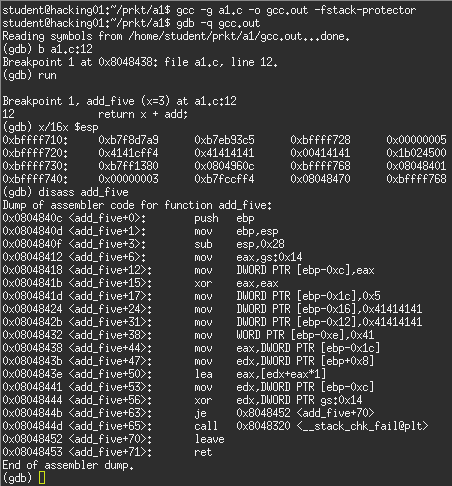
\includegraphics[scale=1]{1_gcc_protector_0.png}
\end{figure}
\begin{figure}[h!]
  \caption{gcc mit Parameter \texttt{no-stack-protector}}
  \label{gcc1}
  \centering
    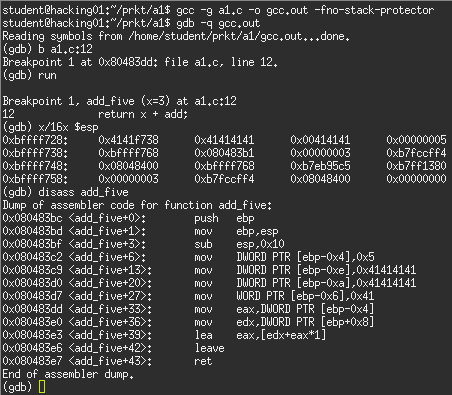
\includegraphics[scale=1]{1_gcc_protector_1.png}
\end{figure}
\begin{figure}[h!]
  \caption{g++ mit Parameter \texttt{stack-protector}}
  \label{gpp0}
  \centering
    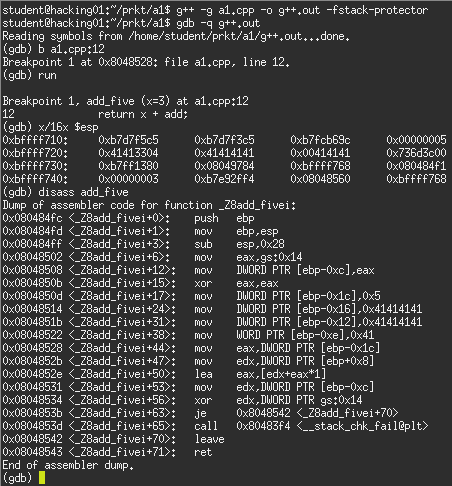
\includegraphics[scale=1]{2_gpp_protector_0.png}
\end{figure}
\begin{figure}[h!]
  \caption{g++ mit Parameter \texttt{no-stack-protector}}
  \label{gpp1}
  \centering
    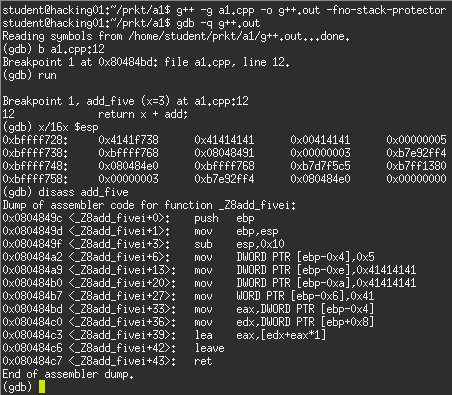
\includegraphics[scale=1]{2_gpp_protector_1.png}
\end{figure}


\section{Aufgabe 2}
\subsection{src\_audit\_1.c}
\subsection{src\_audit\_2.c}
\subsection{src\_audit\_3.c}
\section{Aufgabe 3}
\section{Aufgabe 3}
\section{Aufgabe 4}
\section{Aufgabe 5}
\section{Aufgabe 6}

\end{document}
